\section{有限群表示论}

参见肖梁、Artin.

A matrix representation of a group $G$ is a homomorphism
\[
R:G\to \mathrm{GL}_{n}
\]
from $G$ to one of the complex general linear groups. The number $n$ is the dimension of the representation.

We use the notation $R_g$ instead of $R(g)$ for the image of a group element $g$. Each $R_g$ is an invertible matrix, and the statement that $R$ is a homomorphism reads
\[
R_{g h}=R_g R_h .
\]
If a group is given by generators and relations, say $\left\langle x_1, \ldots, x_n \mid r_1, \ldots, r_k\right\rangle$, a matrix representation can be defined by assigning matrices $R_{x_1}, \ldots, R_{x_n}$ that satisfy the relations. For example, the symmetric group $S_3$ can be presented as $\left\langle x, y \mid x^3, y^2, x y x y\right\rangle$, so a representation of $S_3$ is defined by matrices $R_x$ and $R_y$ such that $R_x^3=I, R_y^2=I$, and $R_x R_y R_x R_y=I$. Some relations in addition to these required ones may hold.

\subsection{Defintions of linear represention, homomorphism of representations (\texorpdfstring{$G$}{G} -linear map), isomorphism of representations, subrepresentation, direct sum of representations, complementary representation, irreducible, tensor product, dual representations}

\begin{figure}[H]
\centering
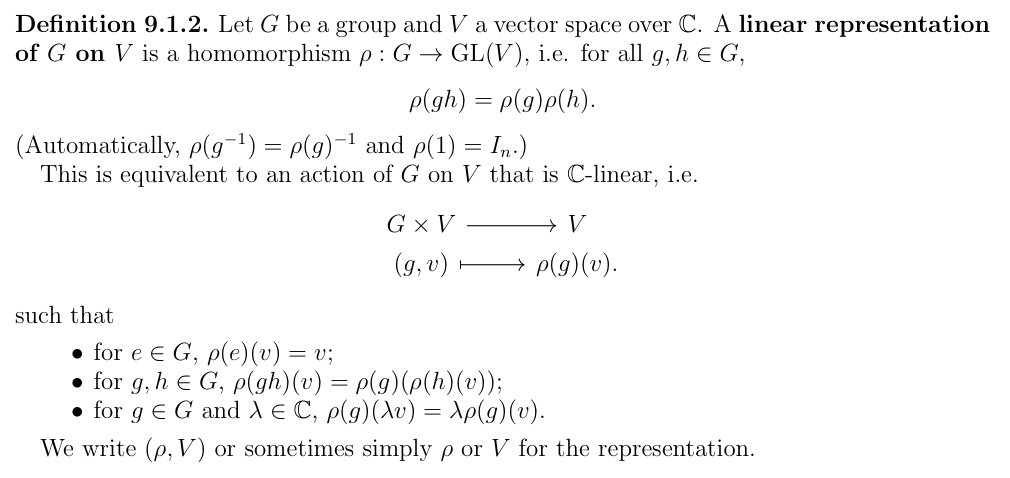
\includegraphics[width=\textwidth]{有限群表示论-2025032521.png}
% \caption{}
\label{}
\end{figure}
\begin{figure}[H]
\centering
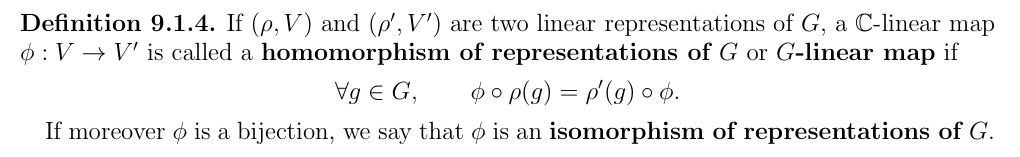
\includegraphics[width=\textwidth]{1-有限群表示论-2025032521.png}
% \caption{}
\label{}
\end{figure}
\begin{figure}[H]
\centering
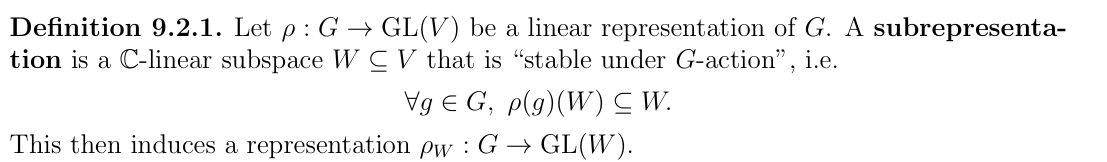
\includegraphics[width=\textwidth]{2-有限群表示论-2025032521.png}
% \caption{}
\label{}
\end{figure}
\begin{figure}[H]
\centering
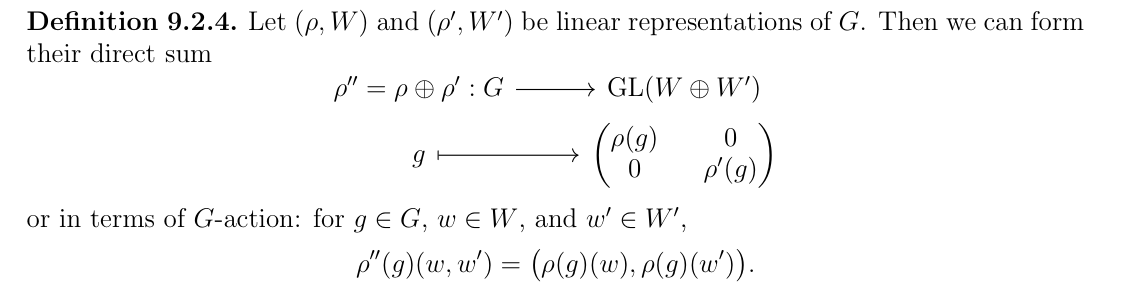
\includegraphics[width=\textwidth]{3-有限群表示论-2025032521.png}
% \caption{}
\label{}
\end{figure}
\begin{figure}[H]
\centering
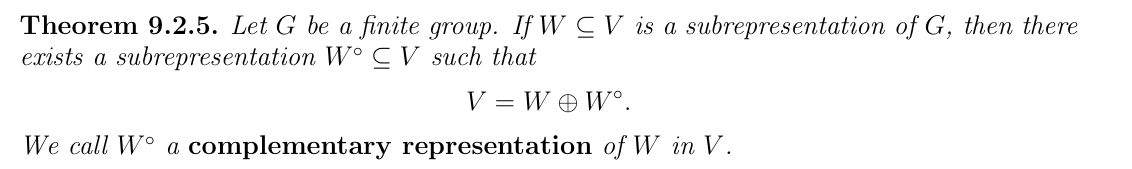
\includegraphics[width=\textwidth]{4-有限群表示论-2025032521.png}
% \caption{}
\label{}
\end{figure}
\begin{figure}[H]
\centering
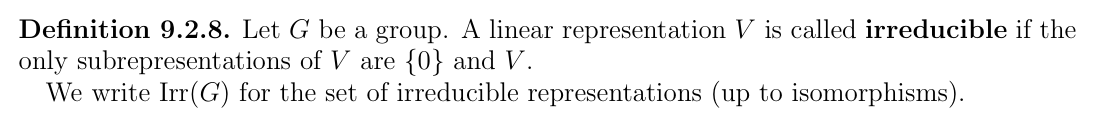
\includegraphics[width=\textwidth]{5-有限群表示论-2025032521.png}
% \caption{}
\label{}
\end{figure}

\begin{note}
If $G$ is finite, then any finite dimensional representation $V$ is "completely reducible".
\begin{figure}[H]
\centering
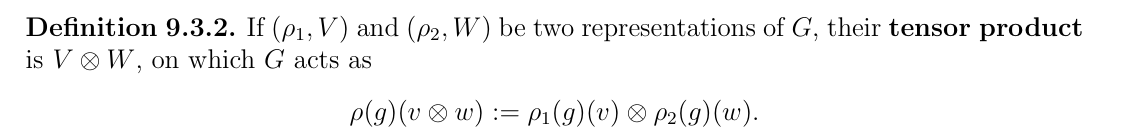
\includegraphics[width=\textwidth]{6-有限群表示论-2025032521.png}
% \caption{}
\label{}
\end{figure}
\begin{figure}[H]
\centering
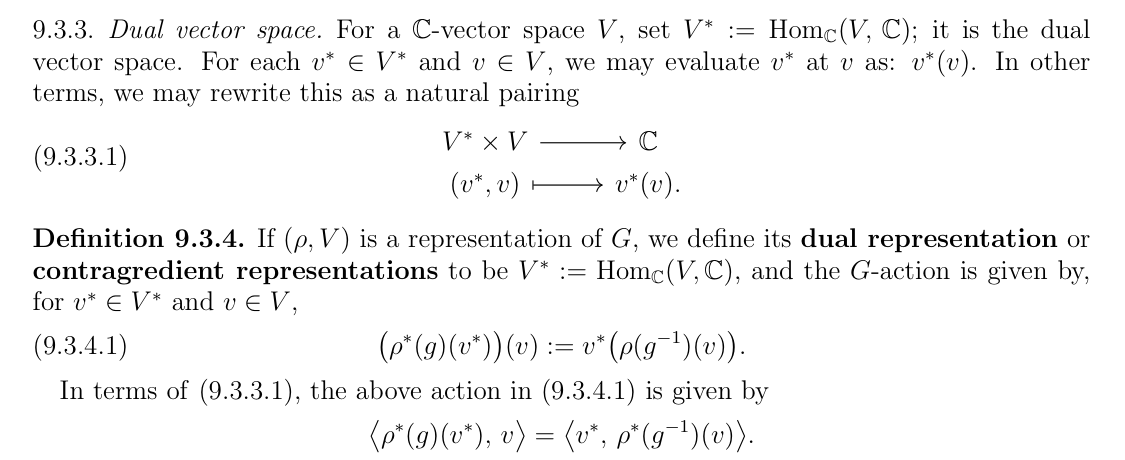
\includegraphics[width=\textwidth]{7-有限群表示论-2025032521.png}
% \caption{}
\label{}
\end{figure}
\begin{figure}[H]
\centering
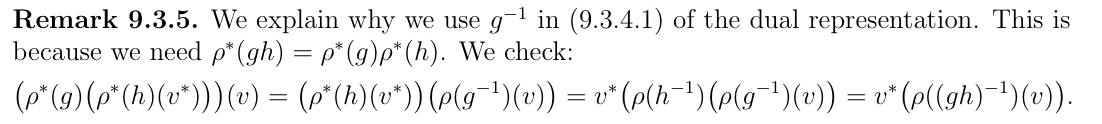
\includegraphics[width=\textwidth]{8-有限群表示论-2025032521.png}
% \caption{}
\label{}
\end{figure}
\begin{figure}[H]
\centering
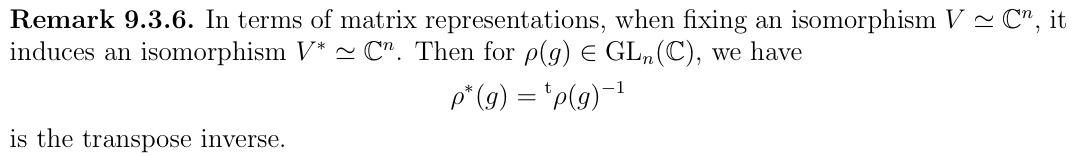
\includegraphics[width=\textwidth]{9-有限群表示论-2025032521.png}
% \caption{}
\label{}
\end{figure}
\end{note}
\subsection{A construction of homomorphism between two linear representations of a finite group \texorpdfstring{$G$}{G}}

\begin{figure}[H]
\centering
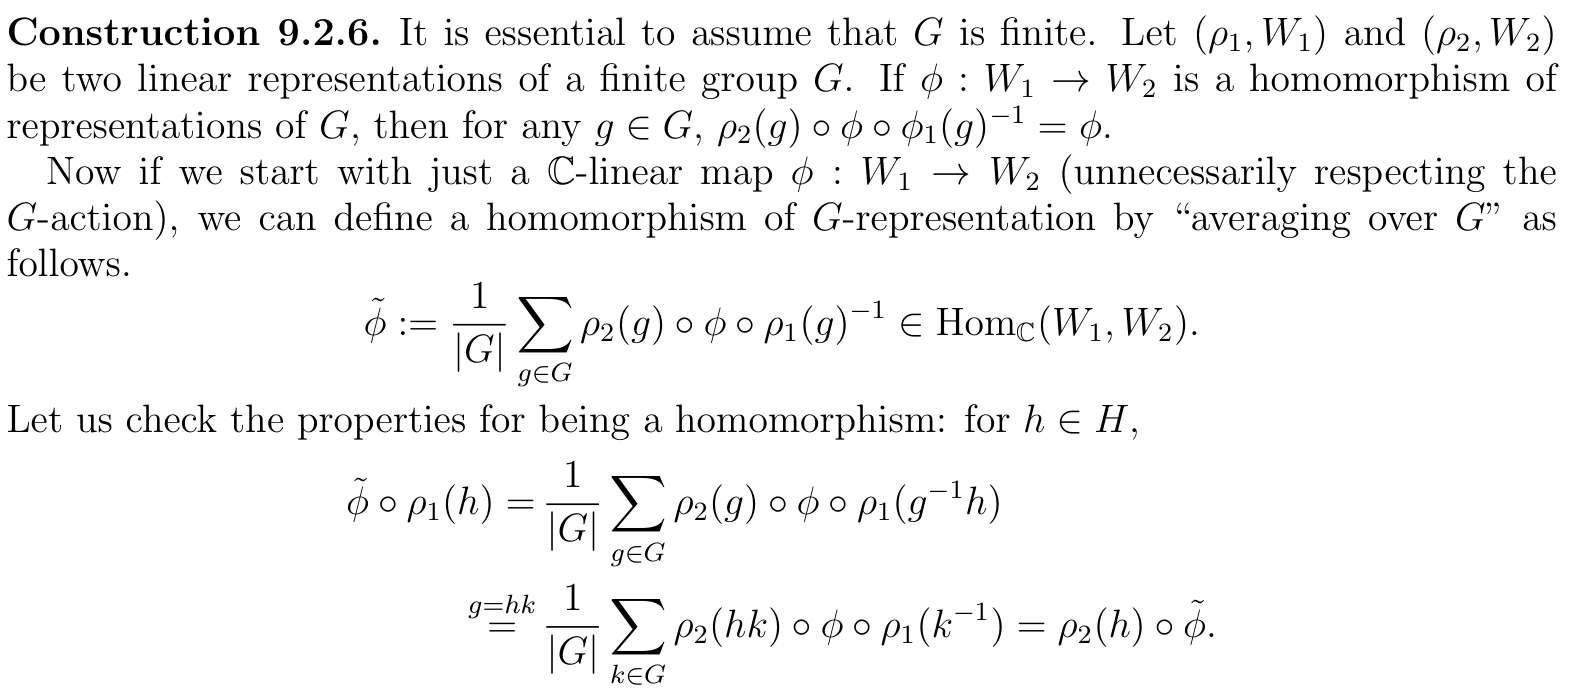
\includegraphics[width=\textwidth]{有限群表示论-2025032601.png}
% \caption{}
\label{}
\end{figure}
\begin{figure}[H]
\centering
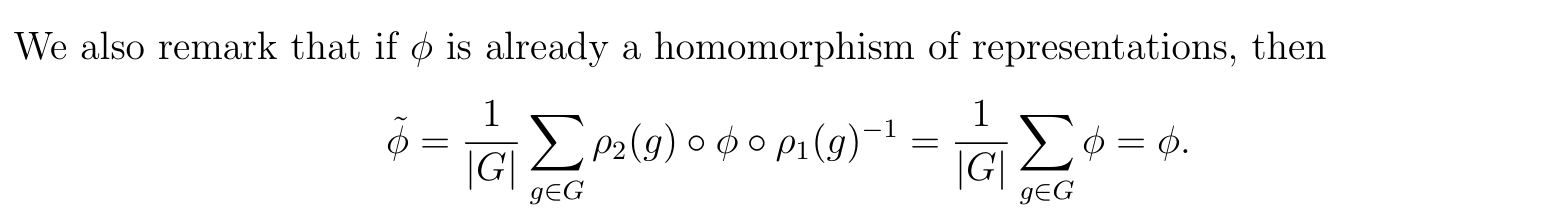
\includegraphics[width=\textwidth]{1-有限群表示论-2025032601.png}
% \caption{}
\label{}
\end{figure}

\subsection{Unitary representations of finite groups}

There is a natural question: can we find a \underline{"good"} matrix representation for a given representation $\rho$ of $G$? Here "good" means there is a positive definite Hermitian form on $V$ so that every $g\in G$ preserves this Hermitian form; and thus the image of $\rho_{\phi}(G)$ in $\mathrm{GL}_{n}(\mathbb{C})$ belongs to the unitary group $\mathrm{U}_n$.

Let $V$ be a Hermitian space -- a complex vector space together with a positive definite Hermitian form $\left< \cdot,\cdot \right>$. A unitary operator $T$ on $V$ is a linear operator with the property
\[
\langle T v, T w\rangle=\langle v, w\rangle\qquad \forall v,w\in V
\]
A representation $\rho:G\to \mathrm{GL}(V)$ on a Hermitian space $V$ is called \textbf{unitary} if $\rho_{g}$ is a unitary operator for every $g$. We can write this condition as
\[
\left< gw,gw \right> = \left< v,w \right> \quad \text{or}\quad \left< \rho_{g}v,\rho_{g}w \right> = \left< v,w \right>
\]
Similarly, a matrix representation $R:G\to \mathrm{GL}_n$ is \textbf{unitary} if $R_{g}\in \mathrm{U}_n,\forall g\in G$. A \textbf{unitary matrix representation} is a homomorphism from $G$ to the unitary group:
\[
R:G\to \mathrm{U}_n
\]
\begin{lemma}
Let $\rho$ be a unitary representation of $G$ on a Hermitian space $V$, and let $W$ be a $G$-invariant subspace. The orthogonal complement $W^{\perp}$ is also $G$-invariant, and $\rho$ is the direct sum of its restrictions to the Hermitian spaces $W$ and $W^{\perp}$. These restrictions are also unitary representations.
\end{lemma}
\begin{proof}
It is true that $V=W \oplus W^{\perp}$. Since $\rho$ is unitary, it preserves orthogonality: If $W$ is invariant and $u \perp W$, then $g u \perp g W=W$. This means that if $u \in W^{\perp}$, then $g u \in W^{\perp}$.
\end{proof}

\subsection{Equivalence of representations}

In matrix terminology, two representation $\varphi$ and $\psi$ are equivalent if there is a fixed invertible matrix $P$ such that
\[
P\varphi(g)P^{-1}=\psi(g)\qquad \forall g\in G
\]
In $FG$ -module terminology, two representation $\varphi$ and $\psi$ are equivalent if there is a fixed $FG$ -module isomorphism $T:V\overset{ \simeq }{ \to }W$ such that
\[
T\circ \varphi(g)=\psi(g)\circ T\qquad \forall g\in G
\]
The linear transformation $T$ or the matrix $P$ above is said to \underline{interwine} the representation $\varphi$ and $\psi$.

\subsection{Characters of representations, class function}

Because they involve several matrices, each of which may have many entries, representations are notationally complicated. The secret to understanding them is to throw out most of the information that the matrices contain, keeping only one essential part, its trace, or character.

Our slogan is: characters determine the representation.
\begin{figure}[H]
\centering
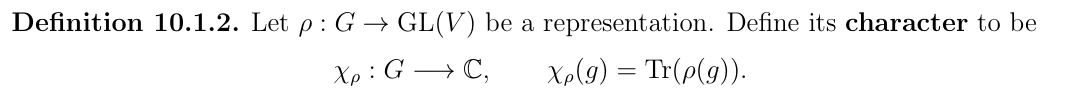
\includegraphics[width=\textwidth]{有限群表示论-2025032522.png}
% \caption{}
\label{}
\end{figure}
\begin{figure}[H]
\centering
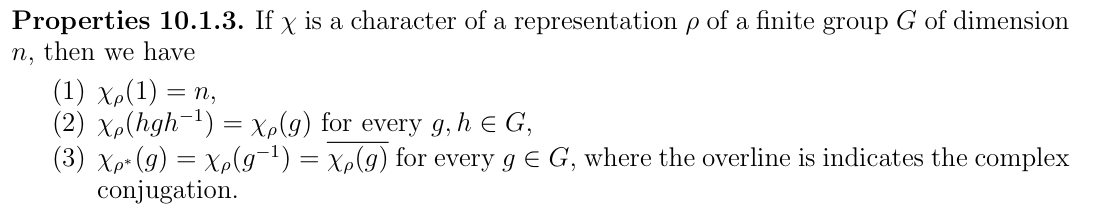
\includegraphics[width=\textwidth]{1-有限群表示论-2025032522.png}
% \caption{}
\label{}
\end{figure}
\begin{figure}[H]
\centering
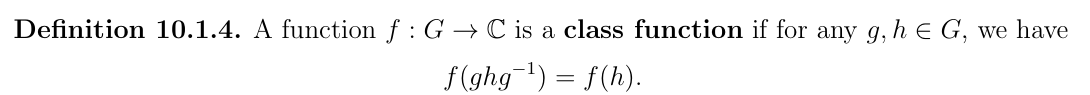
\includegraphics[width=\textwidth]{2-有限群表示论-2025032522.png}
% \caption{}
\label{}
\end{figure}
\begin{figure}[H]
\centering
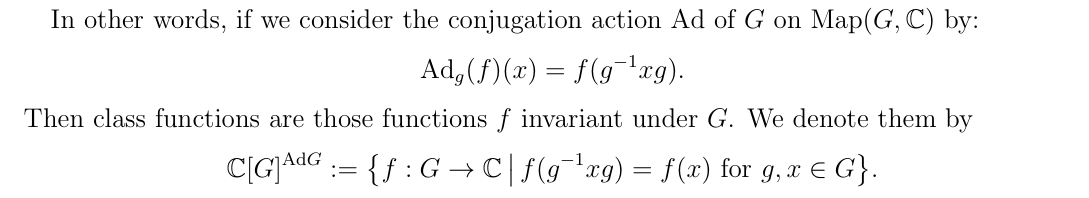
\includegraphics[width=\textwidth]{3-有限群表示论-2025032522.png}
% \caption{}
\label{}
\end{figure}
\begin{figure}[H]
\centering
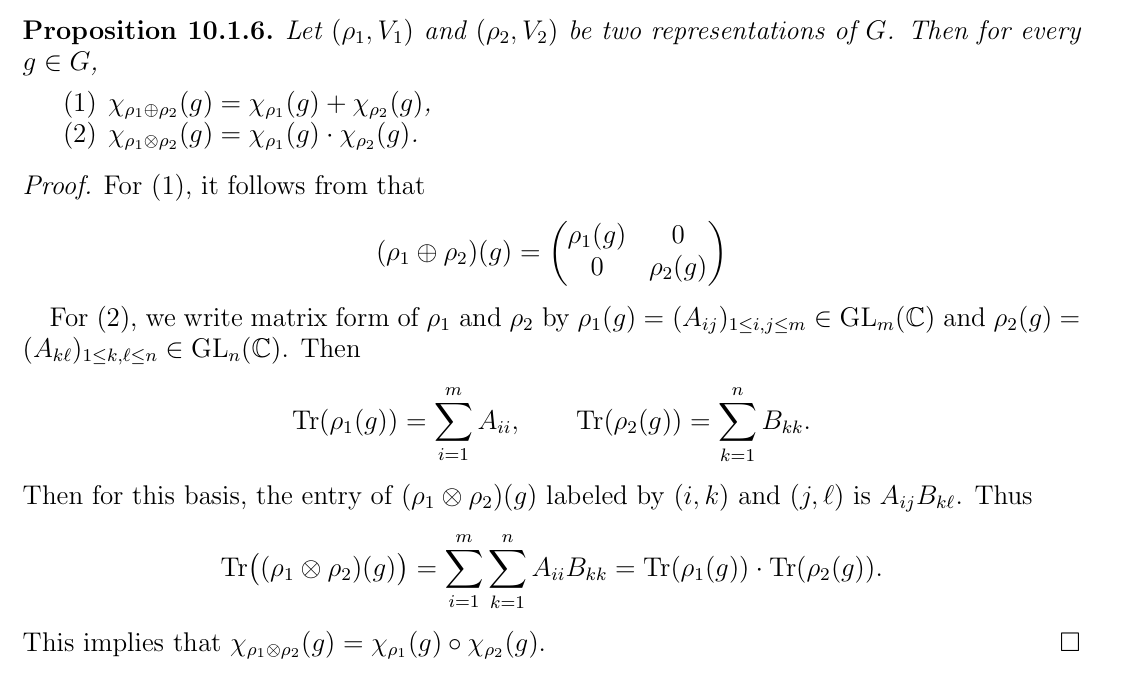
\includegraphics[width=\textwidth]{4-有限群表示论-2025032522.png}
% \caption{}
\label{}
\end{figure}

\subsubsection{Examples}

For $S_3= \left< x,y|x^3,y^3,xyxy \right>$, we have three representaions, $A$, $\Sigma$ and $T$.
\[
A_{x}=\begin{pmatrix}
\cos\frac{2\pi }{3} & -\sin\frac{2\pi}{3} \\
\sin\frac{2\pi}{3} & \cos\frac{2\pi}{3}
\end{pmatrix},\qquad A_{y}=\begin{pmatrix}
1 & 0 \\
0  & -1
\end{pmatrix}
\]
\[
\Sigma_{x}=[1]\qquad \Sigma_{y}=[-1]
\]
\[
T_{x}=[1]\qquad T_{y}=[1]
\]
Then the characters of these representations are displayed below in tabular form.

\begin{table}[h]
	\centering
	\begin{tabular}{|c|c|c|c|c|c|c|}
		\hline
		 & 1 & $x$ & $x^2$ & $y$ & $x y$ & $x^2 y$ \\
		\hline
		$\chi_T$ & 1 & 1 & 1 & 1 & 1 & 1 \\
		\hline
		$\chi_{\Sigma}$ & 1 & 1 & 1 & -1 & -1 & -1 \\
		\hline
		$\chi_A$ & 2 & -1 & -1 & 0 & 0 & 0 \\
		\hline
	\end{tabular}
\end{table}
Several interesting phenomena can be observed in this table:

\begin{itemize}
	\item The rows form orthogonal vectors of length equal to six, which is also the order of $S_3$. The columns are orthogonal too.
	\item $\chi_R(1)$ is the dimension of the representation, also called the dimension of the character.
	\begin{itemize}
		\item Since a representation is a homomorphism, it sends the identity in the group to the identity matrix. So $\chi_R(1)$ is the trace of the identity matrix.
	\end{itemize}
	\item The characters are constant on conjugacy classes.
	\begin{itemize}
		\item The conjugacy classes in $S_3$ are the sets $\{1\},\left\{x, x^2\right\}$, and $\left\{y, x y, x^2 y\right\}$.
		\item This is because conjugate matrices has the same trace.
	\end{itemize}
\end{itemize}

\subsection{Schur's orthogonality}

\begin{figure}[H]
\centering
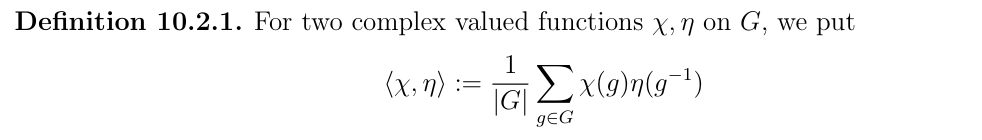
\includegraphics[width=\textwidth]{5-有限群表示论-2025032522.png}
% \caption{}
\label{}
\end{figure}
\begin{figure}[H]
\centering
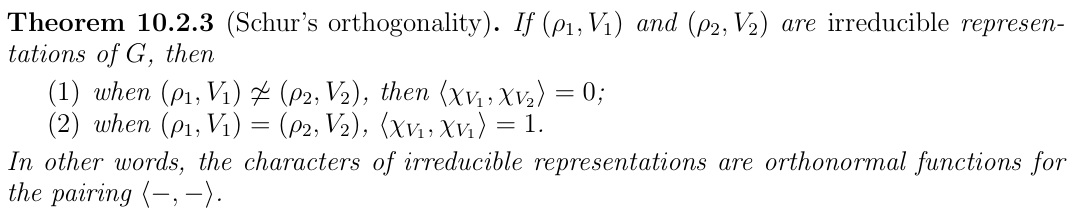
\includegraphics[width=\textwidth]{6-有限群表示论-2025032522.png}
% \caption{}
\label{}
\end{figure}
\begin{figure}[H]
\centering
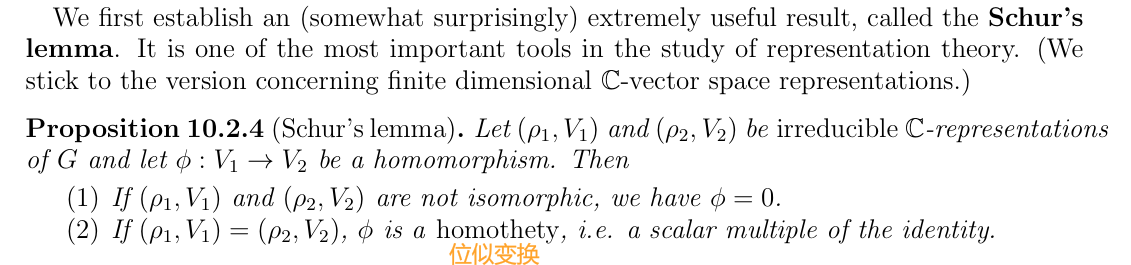
\includegraphics[width=\textwidth]{7-有限群表示论-2025032522.png}
% \caption{}
\label{}
\end{figure}
\begin{figure}[H]
\centering
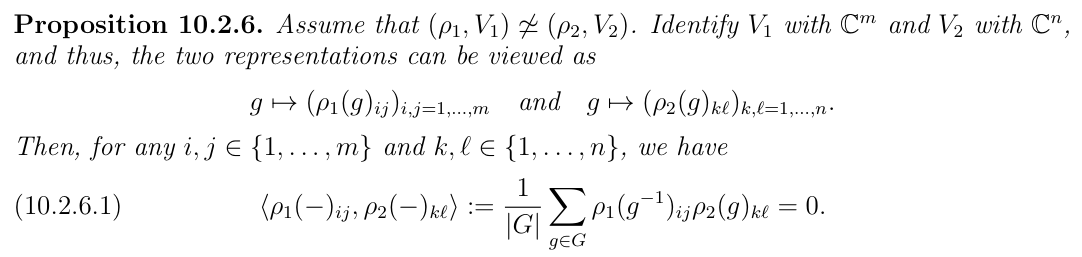
\includegraphics[width=\textwidth]{1-有限群表示论-2025032608.png}
% \caption{}
\label{}
\end{figure}
\begin{figure}[H]
\centering
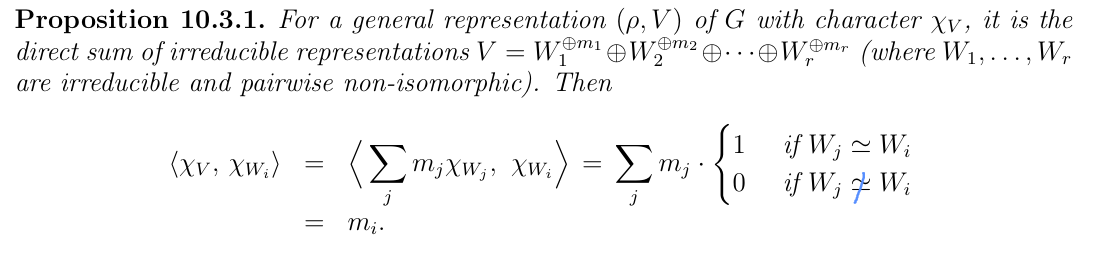
\includegraphics[width=\textwidth]{有限群表示论-2025032608.png}
% \caption{}
\label{}
\end{figure}
\begin{figure}[H]
\centering
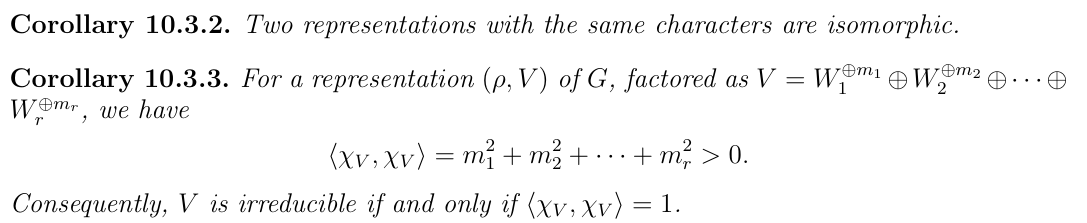
\includegraphics[width=\textwidth]{2-有限群表示论-2025032608.png}
% \caption{}
\label{}
\end{figure}
